%%%%%%%%%%%%%%%%%%%%%%%%%%%%%%%%%%%%% 
%% LE2I beamer template
%% Guillaume Lemaitre, October 2014
%%%%%%%%%%%%%%%%%%%%%%%%%%%%%%%%%%%%% 

\documentclass{beamer}

\usepackage[utf8]{inputenc}
\usepackage[T1]{fontenc} 
\usetheme{le2i} 

%% The amssymb package provides various useful mathematical symbols
\usepackage{amssymb}
%% The amsthm package provides extended theorem environments
\usepackage{amsthm}

%% amsmath for math environment
\usepackage{amsmath}

\DeclareMathOperator*{\argmin}{arg\,min}
\DeclareMathOperator*{\argmax}{arg\,max}
\DeclareMathOperator*{\sign}{sign}

%% figure package
\usepackage{epsf,graphicx}
\usepackage{epstopdf}
\usepackage{subfigure}
\usepackage{transparent}

%% In order to draw some graphs
\usepackage{tikz,xifthen}
\usepackage{tikz-qtree}
\usepackage{adjustbox}
\usetikzlibrary{decorations.pathmorphing}
\usetikzlibrary{fit}
\usetikzlibrary{backgrounds}
\usetikzlibrary{shapes,arrows,shadows}
\usetikzlibrary{calc,decorations.pathreplacing,decorations.markings,positioning}
\usetikzlibrary{snakes,decorations.text,shapes,patterns}
% \usepackage{scalefnt,lmodern,booktabs}

%% Package for cross and tick symbols
\usepackage{pifont}
\newcommand{\tick}{\color{green!60!black!80}\ding{51}}
\newcommand{\cross}{\color{red!60!black!80}\ding{55}}

\title{Image Restoration\\
Frequency Domain}
\author{Guillaume Lemaitre}
%\date{Define the event \\ day\textsuperscript{th} Month Year}

\institute{Universit\'e de Bourgogne} 

%% Uncomment if you want to avoid thousand of bullet inside the menu
% \usepackage{etoolbox}
% \makeatletter
% \patchcmd{\slideentry}{\advance\beamer@xpos by1\relax}{}{}{}
% \def\beamer@subsectionentry#1#2#3#4#5{\advance\beamer@xpos by1\relax}%
% \makeatother

\begin{document}

% Show the title page
\begin{frame}
  \titlepage
\end{frame}

% Show the table of contents
\begin{frame}
  \tableofcontents[sectionstyle=show,subsectionstyle=show,subsubsectionstyle=hide]
\end{frame}

%---------------------
\section{Introduction}
\begin{frame}
\frametitle{Image Restoration}
\framesubtitle{Image restoration vs. image enhancement}
\begin{block}{Image enhancement}
\begin{itemize}
	\item Largely a subjective process
	\item Prior knowledge about the degradation is not a must (sometimes no degradation is involved)
	\item Procedures are heuristic and take advantage of the psychophysical aspects of human visual system
\end{itemize}
\end{block}
\begin{block}{Image restoration}
\begin{itemize}
	\item More an objective process 
	\item Images are degraded
	\item Tires to recover the images by using the knowledge about the degradation
\end{itemize}
\end{block}
\end{frame}
%-----------------
\section{Image Degradation Models}
\begin{frame}
\frametitle{Image degradation}
\begin{block}{Degradation types}
\begin{itemize}
	\item Additive noise	
	\begin{itemize}
		\item Spatial domain restoration (denoising) techniques are preferred 
	\end{itemize}	 
	\item Image blur
	\begin{itemize}
		\item Frequency domain techniques are preferred 
	\end{itemize}
		  
\end{itemize}
\end{block}
\end{frame}
%-----------
\begin{frame}
\frametitle{Image degradation}
\begin{block}{Degradation model}
\begin{itemize}
	\item [] $$g(x,y) = h(x,y)^\ast f(x,y)+\eta(x,y)$$ 
	\begin{itemize}
		\item $f(x,y)$ is the input image free from any degradation
		\item $g(x,y)$ is the degraded image
		\item $h(x,y)$ is the degradation function
		\item $\eta(x,y)$ is additive noise 
		\item $\ast$ is the convolution operator 
		\item In FD : $G(u,v) = H(u,v)F(u,v)+N(u,v)$ 
	\end{itemize}	 	  
\end{itemize}
\end{block}
\begin{block}{Different cases}
\scriptsize{
\begin{itemize}
\item[]$g(x,y)=f(x,y)+\eta(x,y)$
\item[]$g(x,y)=f(x,y)^\ast h(x,y)$
\item[]$g(x,y)= f(x,y)^\ast h(x,y)+ \eta(x,y)$
\end{itemize}
}
\end{block}
\end{frame}
%----------
\begin{frame}
\frametitle{Image Degradation / Restoration}
\begin{block}{Degradation/restoration model}
\centering{
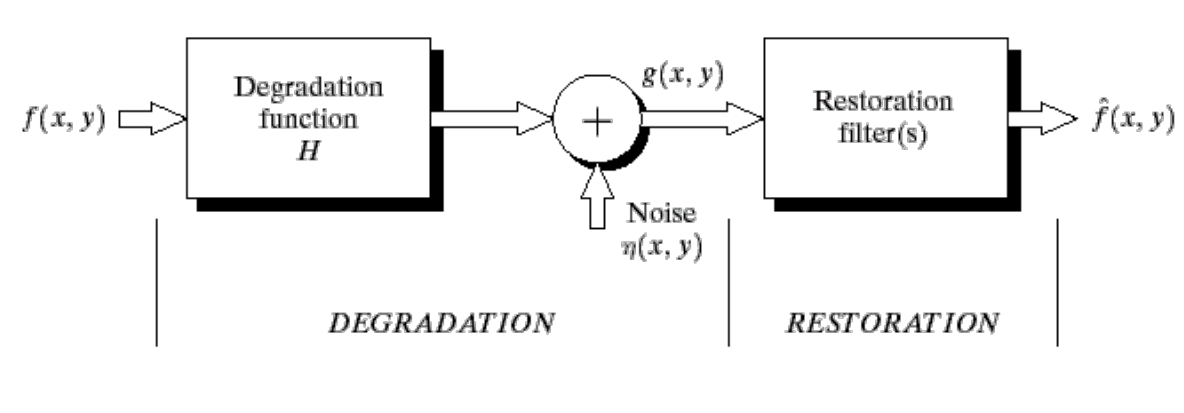
\includegraphics[scale=0.3]{images/L5_DR_model.png}}
\end{block}
\end{frame}
%----------
\subsection{Degradation due to noise}
\begin{frame}
\frametitle{Degradation Due to Noise}
\framesubtitle{Noise models}
\begin{itemize}
	\item White noise
	\item Gaussian noise 
	\item Rayleigh noise 
	\item Erlang (gamma) noise 
	\item Exponential noise 
	\item Uniform noise 
	\item Impulse (salt-and-pepper) noise 
\end{itemize}
\end{frame}
%----------
\begin{frame}	
\frametitle{Degradation Due to noise}
\framesubtitle{Noise models}
\begin{block}{White noise}
\begin{itemize}
	\item Autocorrelation function is an impulse function multiplied by a constant
	$$a(x,y) = \sum^{N-1}_{s=0}\sum^{M-1}_{t=0} \eta(s,t).\eta(s-x,t-y) = N_{0}\delta(x,y)$$
	\item There is no correlation between any two pixels in the noise image
	\item There is no way to predict the next noise value 
	\item The spectrum of the autocorralation function is a constant (White) 
\end{itemize}		
\end{block}
\end{frame}
%----------
\begin{frame}	
\frametitle{Degradation Due to noise}
\framesubtitle{Noise models}
\begin{block}{Gaussian noise}
\begin{itemize}
	\item Noise can be classified according the distribution of the pixel values of the noise image or its normalized histogram
	\item Gaussian noise is characterized by two parameters, mean ($\mu$) and variance ($\sigma^2$)
	$$ p(z) = \frac{1}{\sqrt{2\pi}\sigma}e^{-(z-\mu)^2/2\sigma^2}$$
	\item 70 \% of $z$ values fall in the range $[(\mu-\sigma), (\mu+\sigma)]$
	\item 95 \% of $z$ values fall in the range $[(\mu-2\sigma), (\mu+2\sigma)]$
\end{itemize}		
\end{block}
\end{frame}
%----------
\begin{frame}	
\frametitle{Degradation Due to noise}
\framesubtitle{Noise models}
\begin{block}{Gaussian noise}
\centering{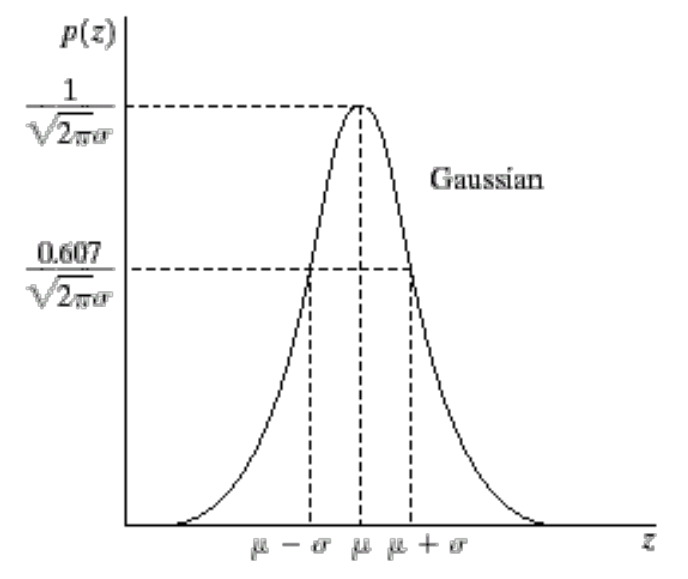
\includegraphics[scale=0.3]{images/L5_DR_GN1.png}}
\end{block}
\end{frame}
%----------
\begin{frame}	
\frametitle{Degradation Due to noise}
\framesubtitle{Noise models}
\begin{block}{Rayleigh noise}
\begin{columns}
\column{0.6\textwidth}
\begin{itemize}
	\item [] 
		\[
 	p(z) = 
  	\begin{cases} 
   	\frac{2}{b}(z-a)e^{-(z-a)^2/b} & \text{for } z \geq a \\
   	0 & \text{for } z < a
  	\end{cases}
	\]
	\item The mean and variance of this density are given by 
	$\mu = a +\sqrt{(\pi b)/4}$, $\sigma^2 = \frac{b(\pi-4)}{4}$
	\item $a$ and $b$ can obtained through mean and variance  
\end{itemize}
\column{0.3\textwidth}
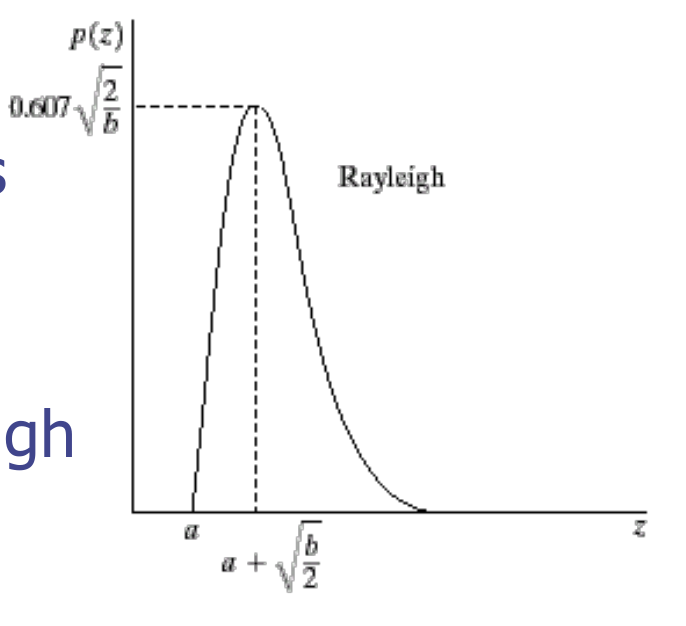
\includegraphics[scale=0.15]{images/L5_DR_RN1.png}
\end{columns}		
\end{block}
\end{frame}
%----------
\begin{frame}	
\frametitle{Degradation Due to noise}
\framesubtitle{Noise models}
\begin{block}{Gamma (erlang) noise}
\begin{columns}
\column{0.6\textwidth}
\begin{itemize}
	\item [] 
		\[
 	p(z) = 
  	\begin{cases} 
   	\frac{a^b z^{b-1}}{(b-1)!}e^{-az} & \text{for } z \geq a \\
   	0 & \text{for } z < a
  	\end{cases}
	\]
	\item The mean and variance of this density are given by
	$\mu = b/a$, $\sigma^2 = b/a^2$
	\item $a$ and $b$ can obtained through mean and variance  
\end{itemize}
\column{0.3\textwidth}
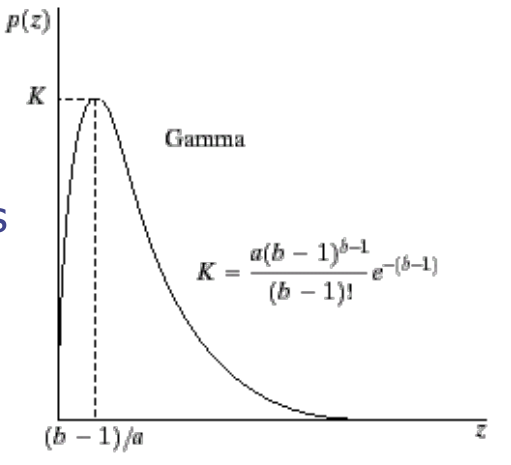
\includegraphics[scale=0.23]{images/L5_DR_EN1.png}
\end{columns}		
\end{block}
\end{frame}
%----------
\begin{frame}	
\frametitle{Degradation Due to noise}
\framesubtitle{Noise models}
\begin{block}{Exponential noise}
\begin{columns}
\column{0.6\textwidth}
\begin{itemize}
	\item [] 
		\[
 	p(z) = 
  	\begin{cases} 
   	ae^{-az} & \text{for } z \geq a \\
   	0 & \text{for } z < a
  	\end{cases}
	\]
	\item The mean and variance of this density are given by
	$\mu = 1/a$, $\sigma^2 = 1/a^2$
	\item Special case of Erlang \textit{pdf} with $b=1$  
\end{itemize}
\column{0.3\textwidth}
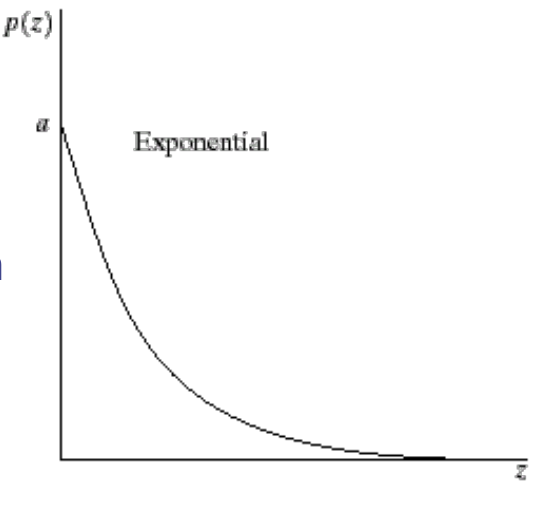
\includegraphics[scale=0.23]{images/L5_DR_ExpN1.png}
\end{columns}		
\end{block}
\end{frame}
%----------
\begin{frame}	
\frametitle{Degradation Due to noise}
\framesubtitle{Noise models}
\begin{block}{Uniform noise}
\begin{columns}
\column{0.6\textwidth}
\begin{itemize}
	\item [] 
		\[
 	p(z) = 
  	\begin{cases} 
   	\frac{1}{b-a} & \text{if } a\leq z \geq b \\
   	0 & \text{Otherwie } 
  	\end{cases}
	\]
	\item The mean and variance of this density are given by
	$\mu = (a+b)/2$, $\sigma^2 = (b-a)^2/12$  
\end{itemize}
\column{0.3\textwidth}
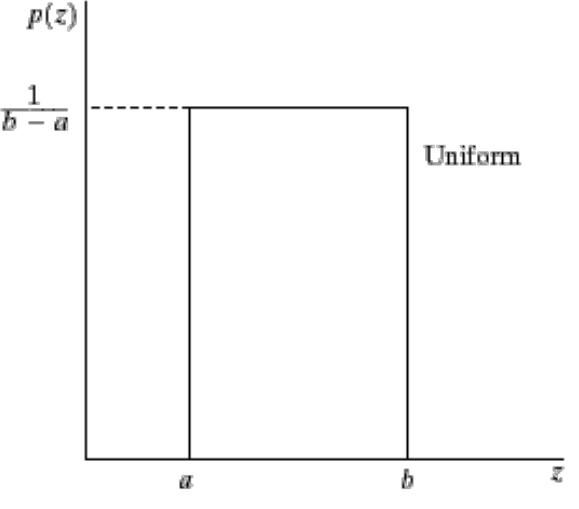
\includegraphics[scale=0.22]{images/L5_DR_UN1.png}
\end{columns}		
\end{block}
\end{frame}
%----------
\begin{frame}	
\frametitle{Degradation Due to noise}
\framesubtitle{Noise models}
\begin{block}{Impulse (salt-and-pepper) noise}
\begin{columns}
\column{0.6\textwidth}
\scriptsize{
\begin{itemize}
	\item [] 
		\[
 	p(z) = 
  	\begin{cases} 
   	P_{a} & \text{for } z=a \\
   	P_{b} & \text{for } z=b \\
   	0 & \text{otherwise} 
  	\end{cases}
	\]
	\item If either $P_{a}$ or $P_{b}$ is zero, the impulse noise is called unipolar
	\item $a$ and $b$ usually are extreme values because impulse corruption is usually large compared with the strength of the image signal
	\item It is the only type of noise that can be distinguished from others visually
\end{itemize}
}
\column{0.3\textwidth}
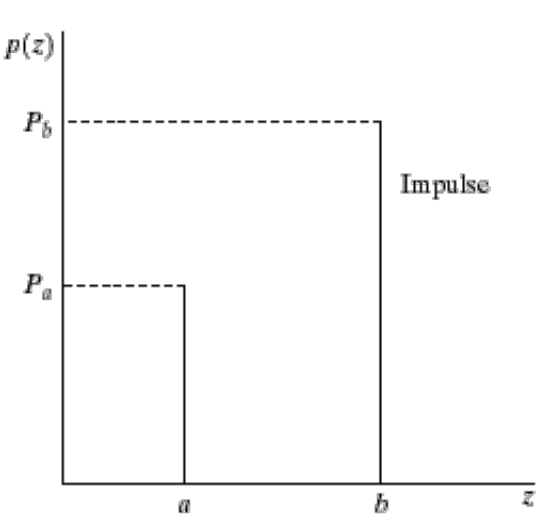
\includegraphics[scale=0.22]{images/L5_DR_SP1.png}
\end{columns}		
\end{block}
\end{frame}
%--------
\begin{frame}
\frametitle{Degradation Due to Noise}
\framesubtitle{Noise models}
\begin{block}{Noise in practice}
\begin{itemize}
\item \textbf{Gaussian noise:} electronic circuit noise and sensor noise due to poor illumination or high temperature
\item \textbf{Rayleigh noise:} range imaging 
\item \textbf{Erlang noise:} laser imaging
\item \textbf{Impulse noise:}  quick transients take place during imaging
\item \textbf{Uniform noise:} used in simulations
\end{itemize}
\end{block}
\end{frame}
%----------
\begin{frame}
\frametitle{Degradation Due to Noise}
\framesubtitle{Noise example}
\begin{columns}
\column{0.2\textwidth}
\centering{
\includegraphics[scale=0.2]{images/L5-ex-ori.png}}
\column{0.8\textwidth}
\centering{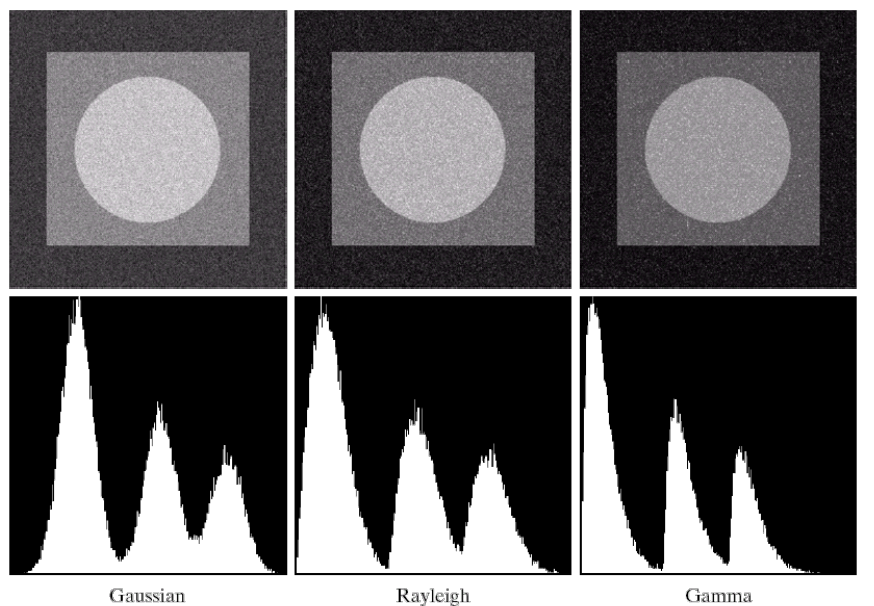
\includegraphics[scale=0.38]{images/L5-ex-GRG.png}}
\end{columns}
\end{frame}
%----------
\begin{frame}
\frametitle{Degradation Due to Noise}
\framesubtitle{Noise example}
\begin{columns}
\column{0.2\textwidth}
\centering{
\includegraphics[scale=0.2]{images/L5-ex-ori.png}}
\column{0.8\textwidth}
\centering{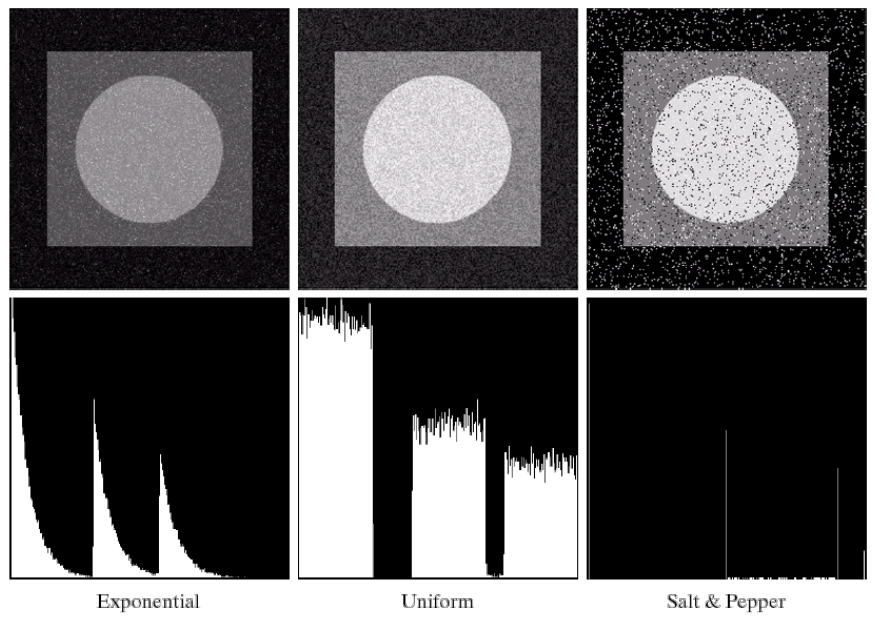
\includegraphics[scale=0.38]{images/L5-ex-EUS.png}}
\end{columns}
\end{frame}
%----------
\section{Periodic Noise}
\begin{frame}	
\frametitle{Degradation Due to Noise}
\framesubtitle{Periodic Noise}
\begin{itemize}
	\item Arises typically from electrical or electromechanical interference during image acquisition
	\item It can be observed by visual inspection both in the spatial and frequency domain 
	\item But only the spatial domain will be considered
	\item Parameters can be estimated by inspection of the spectrum
\end{itemize}
\begin{block}{How to estimate the noise \textit{pdf}}
\scriptsize{
\begin{itemize}
	\item Sensor specifications
	\item Capture a set of images of plain environment, if imaging sensors are available 
	\item If only noisy images are available, \textit{pdf} parameters can be estimated from small patches of constant regions of the noisy image
\end{itemize}
}
\end{block}
\end{frame}
%----------
\begin{frame}
\frametitle{Degradation Due to Noise}
\framesubtitle{Estimation of noise parameters}
\begin{itemize}
	\item Commonly, only mean and variance need to be estimated 
	\item Considering a sub-image with plain scene $S$, 
	$$ \hat{\mu} = \frac{1}{N_{s}} \sum_{(x_{i},y_{i})\in S} z(x_{i}, y_{i})$$ 
	$$ \hat{\sigma_{1}^{2}} = \frac{1}{N_{s}}\sum_{(x_{i},y_{i})\in S}(z(x_{i},y_{i})- \hat{\mu})^2$$ 
\end{itemize}
\end{frame}
%----------
\section{De-Noising}
\subsection{Mean filter}
\begin{frame}
\frametitle{De-Noising}
\begin{block}{Mean filter}
\scriptsize{
$g(x,y)$ is the corrupted image and $S_{x,y}$ is the mask
\begin{itemize}
	\item Arithmetic mean filter 
	$$\hat{f}(x,y) = \frac{1}{mn}\sum_{(s,t)\in S_{x,y}} g(s,t)$$
	\item Geometric mean filter $\rightarrow$ Trends to preserve more details
	$$ \hat{f}(x,y) = \left[ \prod_{\substack{(s,t)\in S_{xy}}} g(s,t)\right] ^\frac{1}{mn}$$
	\item Harmonic mean filter $\rightarrow$ Works well for salt noise but fails for pepper noise
	$$\hat{f}(x,y) = \frac{mn}{\sum\limits_{(x_{i},y_{i})\in S_{xy}} \frac{1}{g(s,t)}} $$ 	
	
\end{itemize}
}
\end{block}

\end{frame}
%----------
\begin{frame}
\frametitle{De-Noising}
\begin{block}{Mean filter}
\begin{itemize}
	\item Contraharmonic mean filter 
	$$\hat{f}(x,y) = \frac{\sum\limits_{(s,t)\in S_{xy}} g(s,t)^{Q+1}}{\sum\limits_{(s,t)\in S_{xy}} g(s,t)^Q}$$
	\begin{itemize}
		\item $Q$ is order of the filter 
		\item $Q > 0 $ $\rightarrow$ pepper noise
		\item $Q < 0 $ $\rightarrow$ salt noise
		\item $Q = 0 $ $\rightarrow$ arithmetic mean filter 
		\item $Q = -1 $ $\rightarrow$ harmonic mean filter
	\end{itemize}	 		
\end{itemize}
\end{block}
\end{frame}
%----------
\begin{frame}
\frametitle{De-Noising}
\begin{block}{Mean filter}
\scriptsize{From right to left and up to bottom : original image, corrupted with Gaussian noise, mean filtering, and geometric mean filtering}\\
\centering{
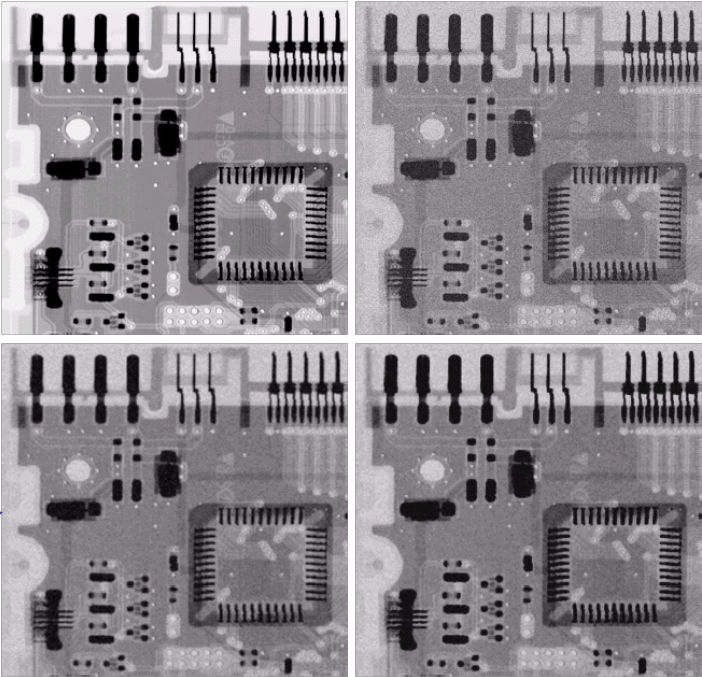
\includegraphics[scale=0.3]{images/L5_ex_Dn_mean1.png}
}
\end{block}
\end{frame}
%----------
\begin{frame}
\frametitle{De-Noising}
\begin{block}{Mean filter}
\scriptsize{From right to left and up to bottom : corrupted with pepper noise, corrupted with salt noise, Contraharmonic filter $Q = 1.5$, Contraharmonic filter $Q = -1.5$}\\
\centering{
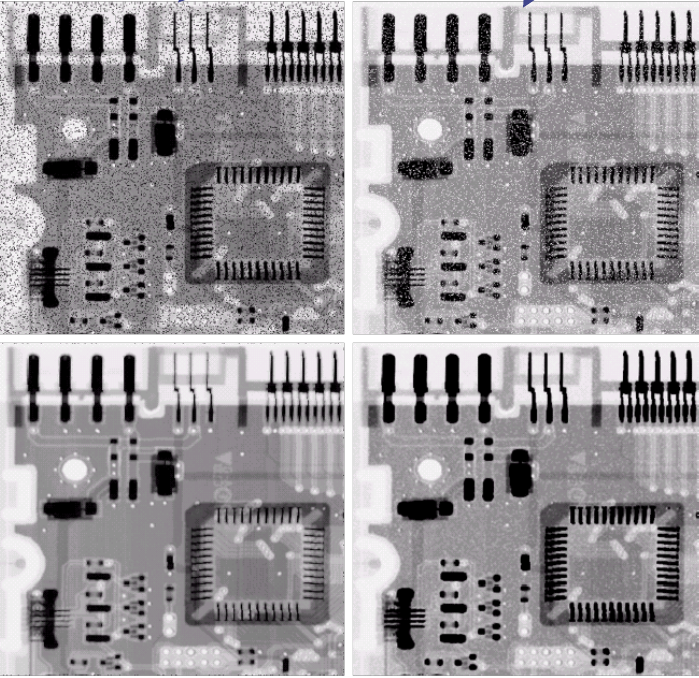
\includegraphics[scale=0.3]{images/L5_ex_Dn_mean2.png}
}
\end{block}
\end{frame}
%----------
\begin{frame}
\frametitle{De-Noising}
\begin{block}{Mean filter}
\begin{itemize}
	\item \scriptsize{Selecting the wrong sign for Contraharmonic filter, from right to left: Contraharmonic filter $Q = -1.5$, Contraharmonic filter $Q = +1.5$}
	\item [] 
\centering{
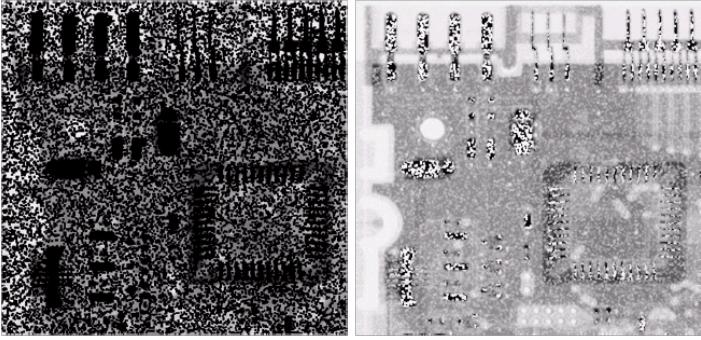
\includegraphics[scale=0.32]{images/L5_ex_Dn_mean3.png}
}
\end{itemize}
\end{block}
\end{frame}
%----------
\subsection{Median filter}
\begin{frame}
\frametitle{De-Noising}
\begin{block}{Median filter}
\begin{itemize}
	\item[] $$\hat{f}(x,y) = median_{(s,t)\in S_{xy}}{g(s,t)}$$
	\item Median represents the $50^{th}$ percentile of a ranked set of numbers
\end{itemize}
\end{block}
\begin{block}{Max and min filter}
\begin{itemize}
	\item Max filter uses the $100^{th}$ percentile of a ranked set of numbers
	\begin{itemize}
		\item Good for removing pepper noise 
	\end{itemize}
		\item Min filter uses the $1^{th}$ percentile of a ranked set of numbers
	\begin{itemize}
		\item Good for removing salt noise 
	\end{itemize}
\end{itemize}
\end{block}
\end{frame}
%----------
\begin{frame}
\frametitle{De-Noising}
\begin{block}{Median filter example}
\scriptsize{Corrupted image with salt-and-pepper, and one, two and third pass with median filter, respectively}\\
\centering{
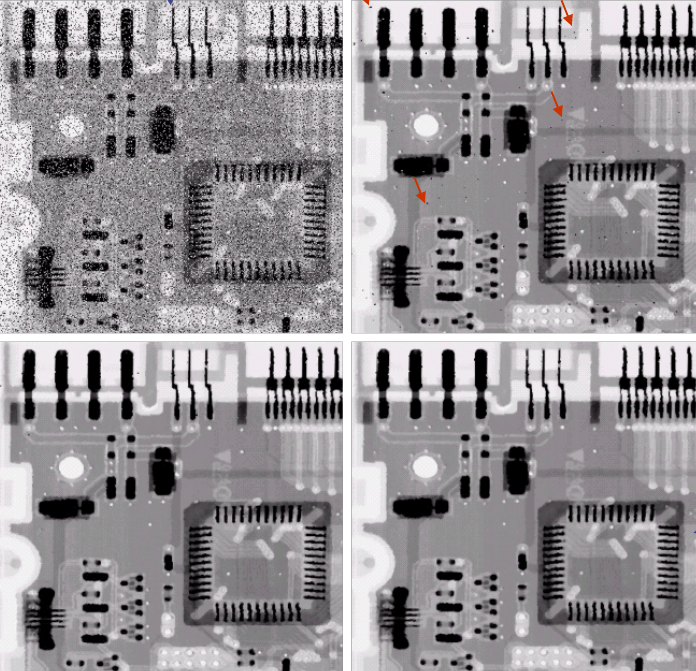
\includegraphics[scale=0.31]{images/L5-ex-median1.png}}
\end{block}
\end{frame}
%----------
\subsection{Max-min filter}
\begin{frame}
\frametitle{De-Noising}
\begin{block}{Max and Min filter example}
\scriptsize{First row: Corrupted images with pepper and salt noise, respectively. Second row: the results of Max and Min filtering, respectively}\\
\centering{
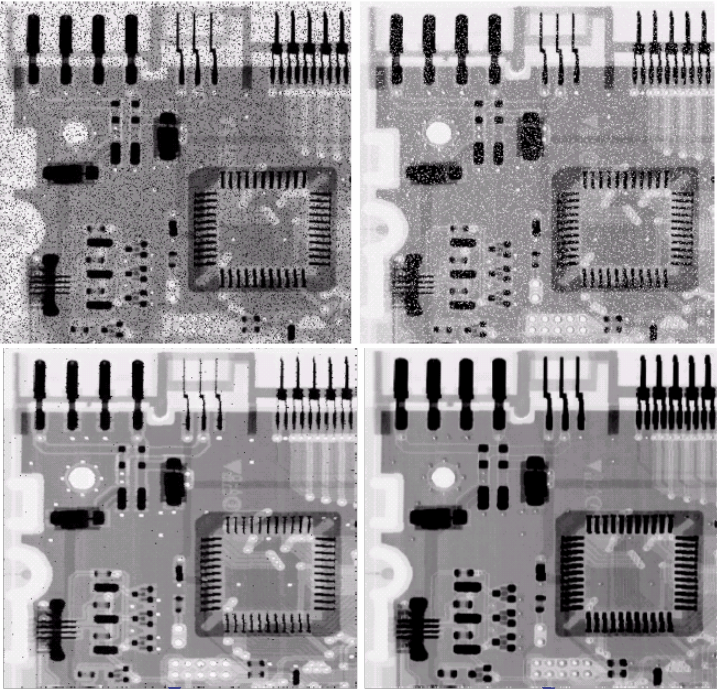
\includegraphics[scale=0.31]{images/L5_ex_MinMax1.png}}
\end{block}
\end{frame}
%----------
\subsection{Midpoint filter}
\begin{frame}
\frametitle{De-Noising}
\begin{block}{Midpoint filter}
\begin{itemize}
	\item[] $$\hat{f}(x,y) = \frac{1}{2}\left[ \max\limits_{(s,t)\in S_{xy}}{g(s,t)} + \min\limits_{(s,t)\in S_{xy}}{g(s,t)} \right]$$
	\item Works best for noise with symmetric \textit{pdf} like Gaussian or uniform noise
\end{itemize}
\end{block}		
\end{frame}
%-----------
\subsection{Alpha trimmed mean filter}
\begin{frame}
\frametitle{De-Noising}
\begin{block}{Alpha trimmed mean filter}
\begin{itemize}
	\item[] $$\hat{f}(x,y) = \frac{1}{mn-d} \sum\limits_{(s,t)\in S_{xy}} g_{r}(s,t)$$
	\item Takes the mean value of the pixels enclosed by an $m \times n$ mask after deleting the pixels with the $d/2$ lowest and highest gray-level values
	\item $g_{r}(s,t)$ represent the remaining $mn-d$ pixels
	\item Useful while dealing with multiple noise (e.g salt-and-pepper and Gaussian) 	
\end{itemize}
\end{block}
\end{frame}
%------------
\begin{frame}
\frametitle{De-Noising - example}
\scriptsize{First column: Corrupted by uniform noise, mean ($5\times 5$), and median ($ 5\times 5$), respectively. Second column: Corrupted by uniform and salt-and-pepper noise, geomean($5\times 5$), and alpha-trimmed mean ($5\times 5$)}\\
\begin{center}
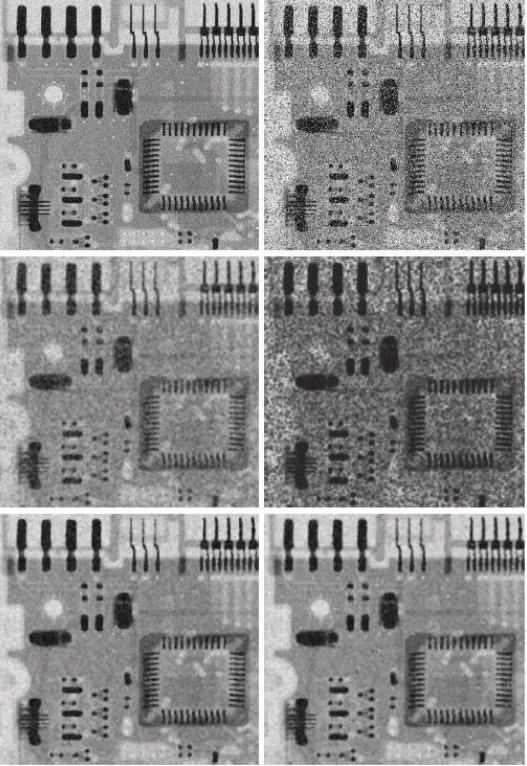
\includegraphics[scale=0.3]{images/L5_ex_allmedian.png}
\end{center}
\end{frame}

%------------
\subsection{Adaptive Filter}
\begin{frame}
\frametitle{De-Noising}
\framesubtitle{Adaptive Filter}
\begin{itemize}
	\item Filters whose behavior changes based on statistical characteristics of the image. 
	\item Two types of adaptive filter: 
	\begin{itemize}
		\item Adaptive, local noise reduction filter 
		\item Adaptive median filter
	\end{itemize}
\end{itemize}
\begin{block}{Adaptive, local noise reduction filter}
Parameters: 
\begin{itemize}
	\item mean($\mu$), average gray level 
	\item variance($\sigma^2$), average contrast
\end{itemize}
Measurements:
\begin{itemize}
	\item noisy image $g(x,y)$, the variance of noise $\sigma_{\eta}^2$, local mean $m_{L}$ in $S_{xy}$, local variance $\sigma_{L}^2$
\end{itemize}

\end{block}
\end{frame}
%----------
\begin{frame}
\frametitle{De-Noising}
\framesubtitle{Adaptive Filter}
\begin{block}{Adaptive, local noise reduction filter}
$$\hat{f}(x,y) = g(x,y)-\frac{\sigma_{\eta}^{2}}{\sigma_{L}^{2}}[g(x,y)-m_{L}] $$
Conditions: 
\begin{itemize}
	\item $\sigma^2_{\eta}$ =  0 $\rightarrow$ Zero noise case 
	\begin{itemize}
	\item Return the value of g(x,y) 
	\end{itemize}	 
	\item $\sigma^{2}_{L} > \sigma^{2}_{\eta}$
	\begin{itemize}
	\item Possible edge and should be preserved 
	\item Return the value close to g(x,y) 
	\end{itemize}	 
	\item $\sigma^{2}_{L} = \sigma^{2}_{\eta}$ 
	\begin{itemize}
	\item When the local area has similar properties with the overall image.
	\item Return arithmetic mean value of the pixels in $S_{xy}$
	\end{itemize}
\end{itemize}
\end{block}
\end{frame}
%----------
\begin{frame}
\frametitle{De-Noising}
\framesubtitle{Adaptive Filter}
\begin{block}{Adaptive, local noise reduction filter}
\scriptsize{LRUB: Image corrupted by additive Gaussian nois $(\mu, \sigma^2) = (0, 1000)$, arithmetic mean filter, geometric mean filter, and adaptive noise reduction. Filter size = $7\times 7$ }\\
\centering{
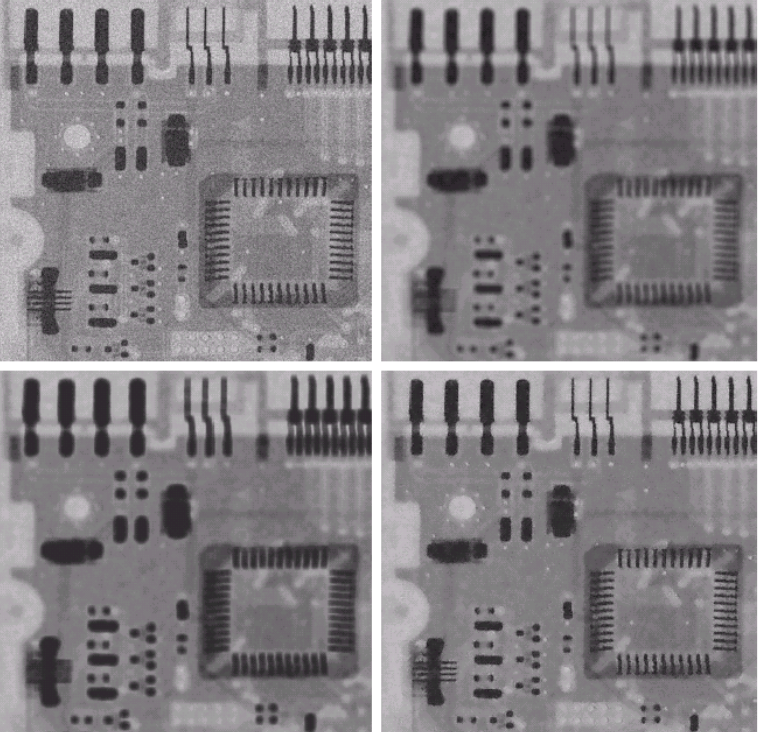
\includegraphics[scale=0.26]{images/L5_ex_LNR1.png}}
\end{block}
\end{frame}
%----------
\begin{frame}
\frametitle{De-Noising}
\framesubtitle{Adaptive Filter}
\begin{block}{Adaptive median filter}
\begin{itemize}
\item Effective for removing salt and pepper noise 
\item The density of the impulse noise can not be too high for median filter compare to adaptive median filter
\item Notations: 
\begin{itemize}
	\item $Z_{min}$, minimum gray value in $S_{xy}$
	\item $Z_{max}$, maximum gray value in $S_{xy}$
	\item $Z_{med}$, median gray value in $S_{xy}$
	\item $Z_{xy}$, gray value of the image at $(x,y)$
	\item $S_{max}$, maximum allowed size of $S_{xy}$
\end{itemize}
\end{itemize}
\end{block}
\end{frame}
%--------
\begin{frame}
\frametitle{De-Noising}
\framesubtitle{Adaptive Filter}
\begin{block}{Adaptive median filter}
\begin{itemize}
\item Two levels of operations: 
\item Level A, {\color{blue} Used to test whether $Z_{med}$ is part of s-and-p noise, if yes, window size is increased}
\begin{itemize}
	\item $A_{1} = Z_{med} - Z_{min}$
	\item $A_{2} = Z_{med} - Z_{max}$
	\item if $A_{1} > 0$ \& $A_{2} < 0$  $\rightarrow$ Level B
	\item else $\rightarrow$ increase $S_{xy}$ size by 2
	\item if window size $\leq S_{max}$ repeat Level A else return $Z_{xy}$
\end{itemize}
\item Level B, {\color{blue} Used to test whether $Z_{xy}$ is part of s-and-p noise, if yes, apply regular median filtering}
\begin{itemize}
	\item $B_{1} = Z_{xy} - Z_{min}$
	\item $B_{2} = Z_{xy} - Z_{max}$
	\item if $B_{1} > 0$ \& $B_{2} < 0$, return $Z_{xy}$ 
	\item else return $Z_{med}$ 
\end{itemize}
\end{itemize}
\end{block}
\end{frame}
%-----------
\begin{frame}
\frametitle{De-Noising}
\framesubtitle{Adaptive Filter}
\begin{block}{Adaptive median filter}
\begin{itemize}
\item[]
\scriptsize{Image corrupted with s-and-p noise, median filter ($7 \times 7$), and adaptive median filtering ($S_{max} = 7$), respectively}\\
\item []
\centering{
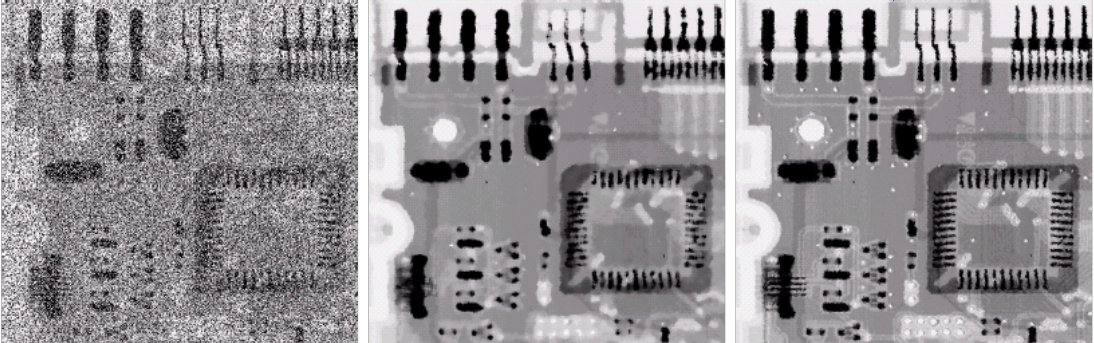
\includegraphics[scale= 0.3]{images/L5_ex_AM1.png}}
\end{itemize}
\end{block}
\end{frame}
%-----------
\section{Periodic noise removal}
\begin{frame}
\frametitle{Periodic noise reduction}
\framesubtitle{Frequency domain Filtering}
\begin{itemize}
\item Lowpass and highpass filters for image enhancement
\item Bandreject, bandpass and notch filters for periodic noise reduction or removal
\end{itemize}
\begin{block}{Bandreject filters}
\begin{itemize}
\item Bamdreject filters remove or attenuate a band of frequencies about the origin of the Fourier transform
\item Ideal, Butterworth, Gaussian bandreject filters
\end{itemize}
\end{block}
\end{frame}
%------------
\begin{frame}
\frametitle{Periodic noise reduction}
\begin{block}{Bandreject Ideal filters}
\begin{itemize}
\item[] 
	\[
 	H(u,v) = 
  	\begin{cases} 
   	1 & \text{if } D(u,v) < D_{0}-\frac{W}{2} \\
   	0 & \text{if } D_{0}-\frac{W}{2} \leq  D(u,v) \leq D_{0}+\frac{W}{2} \\
   	1 & \text{if } D(u,v) > D_{0}+\frac{W}{2}
  	\end{cases}
	\]
\item[] \centering{
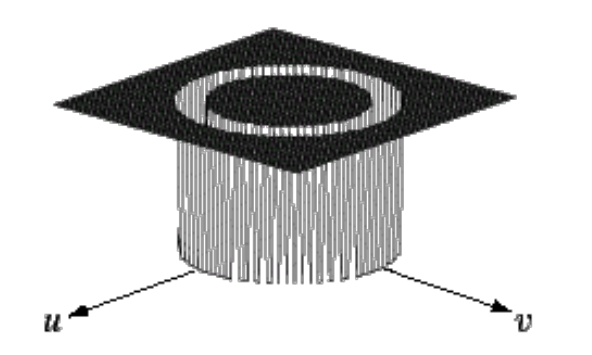
\includegraphics[scale= 0.3]{images/L5_BR_ideal.png}}
\end{itemize}
\end{block}
\end{frame}
%------------
\begin{frame}
\frametitle{Periodic noise reduction}
\begin{block}{Bandreject Butterworth filters}
\begin{itemize}
\item[] 
	\[
 	H(u,v) = \frac{1}{1+\left[ \frac{D(u,v)W}{D^2(u,v)-D_{0}^2}\right]^{2n}}
  	\]
\item[] \centering{
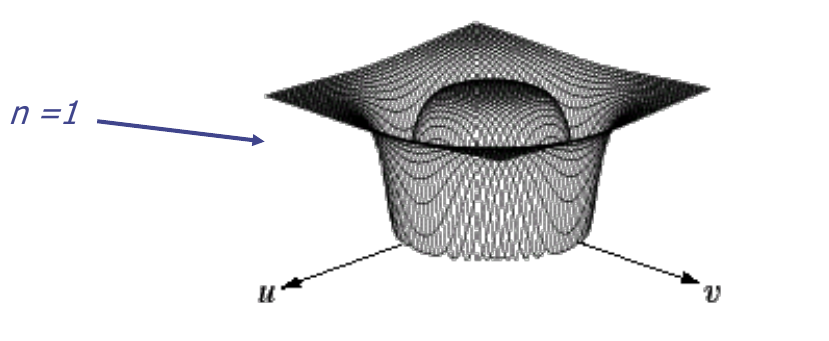
\includegraphics[scale= 0.3]{images/L5_BR_BW.png}}
\end{itemize}
\end{block}
\end{frame}
%------------
\begin{frame}
\frametitle{Periodic noise reduction}
\begin{block}{Bandreject Guassian filters}
\begin{itemize}
\item[] 
	\[
 	H(u,v) = 1 - e^\frac{-1}{2}\left[\frac{D^2(u,v)-D_{0}^2}{D(u,v)W}\right]
  	\]
\item[] \centering{
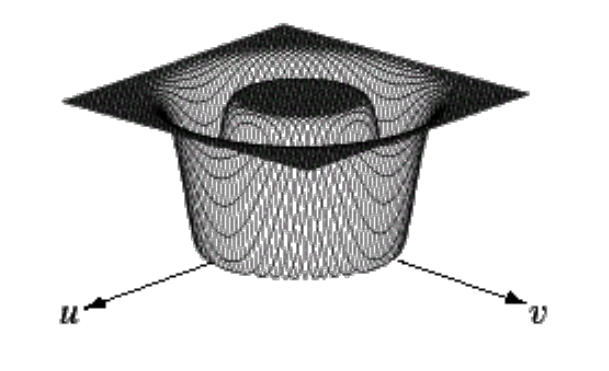
\includegraphics[scale= 0.3]{images/L5_BR_G.png}}
\end{itemize}
\end{block}
\end{frame}
%-------------
\begin{frame}
\frametitle{Periodic noise reduction}
\begin{block}{Bandreject filter}
\begin{itemize}
\item[]Corrupted image by sinusoidal noise and filtered image by Butterworth bandrejected filter
\item[]\centering{
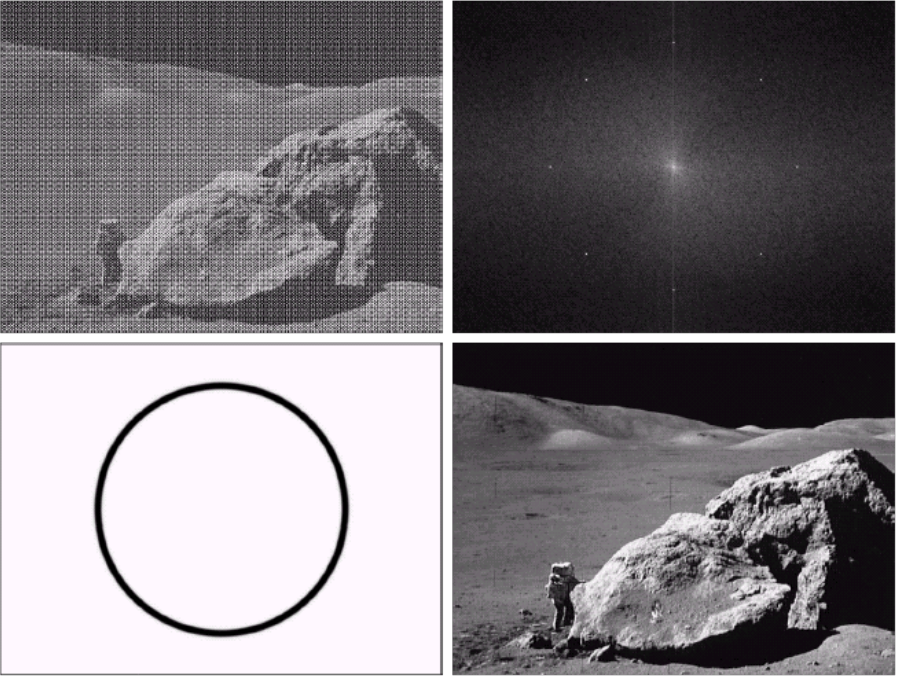
\includegraphics[scale=0.3]{images/L5_ex_BR_BW.png}}
\end{itemize}
\end{block}
\end{frame}
%-------------
\begin{frame}
\frametitle{Periodic noise reduction}
\begin{block}{Bandpass filter}
\begin{itemize}
\item[]Performs opposite of bandreject filter 
\item[]$$ H_{bp}(u,v) = 1 - H_{br}(u,v)$$
\end{itemize}
\end{block}
\begin{block}{Notch filter}
\begin{itemize}
\item Notch filter ejects frequencies in predefined neighborhoods about a center frequency
\item It appears in symmetric pairs about the origin because the Fourier transform of a real valued image is symmetric
\end{itemize}
\end{block}
\end{frame}
%-------------
\begin{frame}
\frametitle{Periodic noise reduction}
\begin{block}{Ideal notch filter}
\begin{itemize}
\item[]
\[
 	H(u,v) = 
  	\begin{cases} 
   	0 & \text{if } D_{1}(u,v) \leq D_{0} \text{or } D_{2}(u,v) \leq D_{0}   \\
   	1 & \text{otherwise }
  	\end{cases}
	\]
	$$D_{1}(u,v) = \left[ (u-M/2-u_{0})^2 + (u-N/2-v_{0})^2 \right]^{1/2}$$
	$$D_{2}(u,v) = \left[ (u-M/2+u_{0})^2 + (u-N/2+v_{0})^2\right]^{1/2}$$
\item[]
\centering{
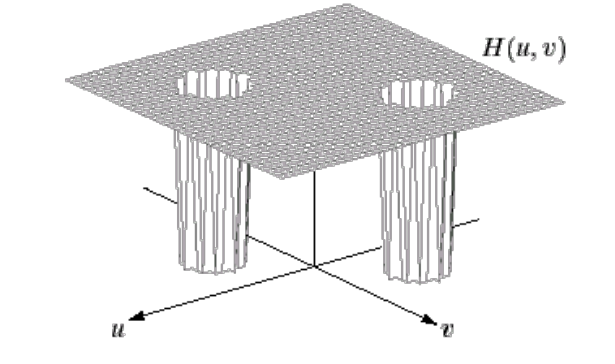
\includegraphics[scale=0.3]{images/L5_N_ideal.png}}
\end{itemize}
\end{block}
\end{frame}
%-----------
\begin{frame}
\frametitle{Periodic noise reduction}
\begin{block}{Butterworth notch filter}
\begin{itemize}
\item[]
	\[
 	H(u,v) = \frac{1}{1+\left[ \frac{D_{0}^2}{D_{1}(u,v)D_{2}(u,v)}\right]^{2n}}
  	\]
\item[]
\centering{
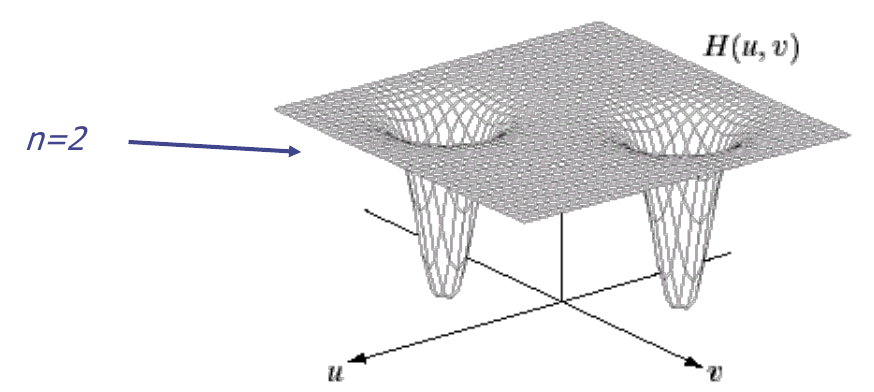
\includegraphics[scale=0.3]{images/L5_N_BW.png}}
\end{itemize}
\end{block}
\end{frame}
%-----------
\begin{frame}
\frametitle{Periodic noise reduction}
\begin{block}{Gaussian notch filter}
\begin{itemize}
\item[]
	\[
 	H(u,v) = 1 - e^\frac{-1}{2}\left[\frac{D_{1}(u,v)D_{2}(u,v)}{D_{0}^2}\right]
  	\]
\item[]
\centering{
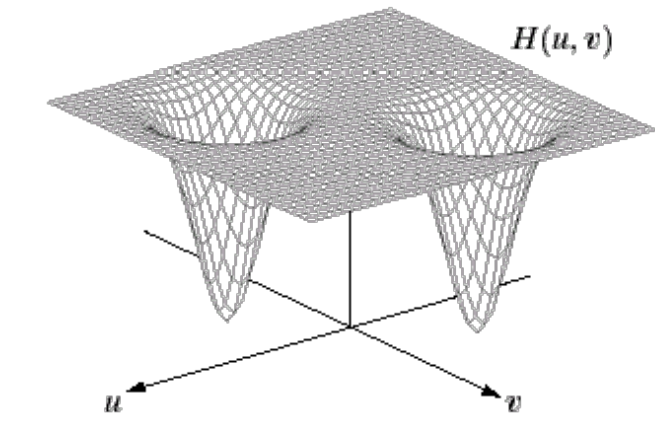
\includegraphics[scale=0.3]{images/L5_N_G.png}}
\end{itemize}
\end{block}
\end{frame}
%-----------
\begin{frame}
\frametitle{Periodic noise reduction}
\begin{block}{Notch filter}
\begin{itemize}
\item Notch filter that pass, rather than suppress: 
$$ H_{np}(u,v) = 1 - H_{nr}(u,v)$$
\item If $u_{0} = v_{0} = 0$,  NR filters become highpass filters
\item If $u_{0} = v_{0} = 0$,  NP filters become lowpass filters
\end{itemize}
\end{block}
\end{frame}
%------------
\begin{frame}
\frametitle{Periodic noise reduction}
\begin{block}{Optimum Notch filter}
\begin{itemize}
\scriptsize{
\item Minimizing the effects of components not presented in estimation of $\eta(x,y)$, by : 
$$ \hat{f}(u,v) = g(x,y) -w(x,y)\hat{\eta}(x,y)$$
\noindent $w(x,y)$ is weighted or modulation function
\item Here the modulation function is a constant within a neighborhood of size $(2a+1)$ by $(2b+1)$ about a point $(x,y)$
\item We optimize its performance by minimizing the local variance of the restored image at the position $(x,y)$

$$\sigma^{2}(x,y) = \frac{1}{(2a+1)(2b+1)} \sum^{a}_{s=-a} \sum^{b}_{t=-b}[\hat{f}(x+s,y+t) - \bar{\hat{f}}(x,y)]^2 $$
$$\bar{\hat{f}}(x,y) = \frac{1}{(2a+1)(2b+1)} \sum^{a}_{s=-a} \sum^{b}_{t=-b} \hat{f}(x+s,y+t)$$
}
\end{itemize}
\end{block}
\end{frame}
%------------
\begin{frame}
\frametitle{Periodic noise reduction}
\begin{block}{Optimum Notch filter}
\begin{itemize}
\scriptsize{
\item Points on or near Edge of the image can be treated by considering partial neighborhoods or by zero padding the borders
$$\sigma^{2}(x,y) = \frac{1}{(2a+1)(2b+1)} \sum^{a}_{s=-a} \sum^{b}_{t=-b}\lbrace [g(x+s,y+t)-w(x+s,y+t)$$
$$\hat{\eta}(x+s,y+t)]- [\bar{g}(x,y) - \overline{w(x,y)\eta(x,y)}]\rbrace^2$$
\item Assumption: $w(x+s, y+t) = w(x,y)$ for $-a \leq s \leq a$ and $-b \leq t \leq b$
\item[] $\Rightarrow$  $\overline{w(x,y)\eta(x,y)} = w(x,y)\bar{\hat{\eta}}(x,y)$
}
\end{itemize}
\end{block}
\end{frame}
%------------
\begin{frame}
\frametitle{Periodic noise reduction}
\begin{block}{Optimum Notch filter}
\begin{itemize}
\item [] 
$$ \Rightarrow \sigma^{2}(x,y) = \frac{1}{(2a+1)(2b+1)} \sum^{a}_{s=-a} \sum^{b}_{t=-b}\lbrace [g(x+s,y+t)- $$
$$w(x,y)\hat{\eta}(x+s,y+t)]- [\bar{g}(x,y) - w(x,y)\bar{\hat{\eta}}(x,y)]\rbrace^2$$
\end{itemize}
\end{block}
\end{frame}
%-----------
\begin{frame}
\frametitle{Periodic noise reduction}
\begin{block}{Optimum Notch filter}
\begin{itemize}
\item To minimize $\sigma^2(x,y)$
\item[] $$\frac{\partial \sigma^2 (x,y)}{\partial w(x,y)} = 0 $$ 
\item[] $$\Rightarrow w(x,y) = \frac{\overline{g(x,y)\hat{\eta}(x,y)} - \bar{g}(x,y)\bar{\hat{\eta}}(x,y)}{\bar{\eta^2}(x,y) - \bar{\eta^2}(x,y)}$$
\end{itemize}
\end{block}
\end{frame}
%----------
\section{Linear, Position-Invariant Degradation}
\begin{frame}
\frametitle{Linear, position-invariant degradation}
\begin{itemize}
	\item[] $$g(x,y) = H[f(x,y)]+\eta(x,y)$$
	\item In the absence of additive noise:
	\begin{itemize}
	\item For scalar values of $a$ and $b$, $H$ is linear, if : 
	$$H[af_{1}(x,y)+bf_{2}(x,y)] = aH[f_{1}(x,y)]+bH[f_{2}(x,y)] $$ 
	\item H is position-invariant if:
	$$ g(x,y) = H[f(x,y)] \Rightarrow H[f(x-\alpha, y-\beta)] = g(x-\alpha, y-\beta)$$	
	\end{itemize}
	\item In the presence of additive noise:
	\begin{itemize}
	\item if H is position invariant: 
	\scriptsize{
	$$ g(x,y) = \int_{-\infty}^{+\infty}\int_{-\infty}^{+\infty} f(\alpha, \beta)h(x-\alpha,y-\beta)d\alpha d\beta +\eta(x,y)$$
	$$ g(x,y) = h(x,y)^{\ast} f(x,y)+\eta(x,y)$$
	$$ G(u,v) = H(u,v)F(u,v)+N(u,v)$$
	}
	\end{itemize}				
\end{itemize}
\end{frame}
%-----------
\begin{frame}
\frametitle{Linear, position-invariant degradation}
\begin{block}{Summary}
\begin{itemize}
\item Linearly spatially-invariant degradation system with additive noise: 
	\begin{itemize}
	\item Spatial domain: Convolution of degradation function with image and addition of noise
	\item Frequency domain: Product of FT of degradation function with image followed by addition of FT of noise
	\end{itemize}
\item Many types of degradation can be approximated by linear, position-invariant processes
\item Extensive tools of linear system theory are available
\item Degradation are modeled as a result of convolution $\Rightarrow$ Restoration, \textbf{image deconvolution} $\Rightarrow$ deconvolution filters
\end{itemize}
\end{block}
\end{frame}
%-----------
\section{Estimating the degradation function}
\begin{frame}
\frametitle{Estimating the degradation function}
\begin{itemize}
	\item Observation
	\item Experimentation 
	\item Mathematical modeling
\end{itemize}
\begin{block}{Estimation by image observation}
\scriptsize{
\begin{itemize}
	\item Gather information from the image itself	
	\item Considering a small section of the image with a strong signal content $g_{s}(x,y)$ construct an un-degradation of this section by using sample gray levels ($\hat{f_{s}}(x, y)$)	
	\item Assuming that the effects of noise is negligible (Strong-signal area):
	$$H_{s}(u,v) = \frac{G_{s}(u,v)}{\hat{F_{s}}(u,v)}$$
	\item Considering the position-invariant assumption, we construct a function $H(u,v)$ on a large scale with the same shape as $H_{s}(u,v)$.
\end{itemize}
}
\end{block}
\end{frame}
%-----------
\begin{frame}
\frametitle{Estimating the degradation function}
\begin{block}{Estimation by experimentation}
\scriptsize{
\begin{itemize}
	\item Gather information using the image acquisition system (if its available)
	\item Imaging of impulse response (small dot of light) with the same system, to obtain impulse response of the degradation
	$$H(u,v) = \frac{G(u,v)}{A}$$
	\noindent $A$ is a constant describing the strength of the impulse
	\item A linear space-invariant system is characterized completely by its impulse response. 
	\item An impulse of light (right) and Image impulse (degraded, left)
	\centering{
	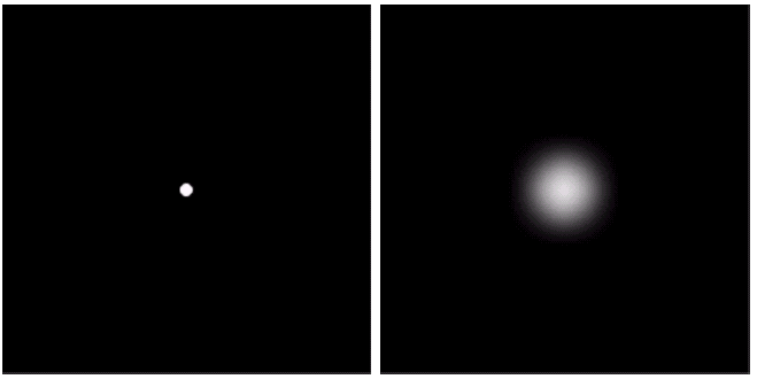
\includegraphics[scale=0.2]{images/L5_EbE.png}}
	\end{itemize}
}
\end{block}
\end{frame}
%-----------
\begin{frame}
\frametitle{Estimating the degradation function}
\begin{block}{Estimation by modeling}
\scriptsize{
\begin{itemize}
	\item E.g: Degradation model proposed for atmospheric turbulence, where $k$ is a constant depending on the nature of turbulence 
	$$H(u,v) = e^{-k(u^2+v^2)^{5/6}}$$
	\noindent
	\centering{
	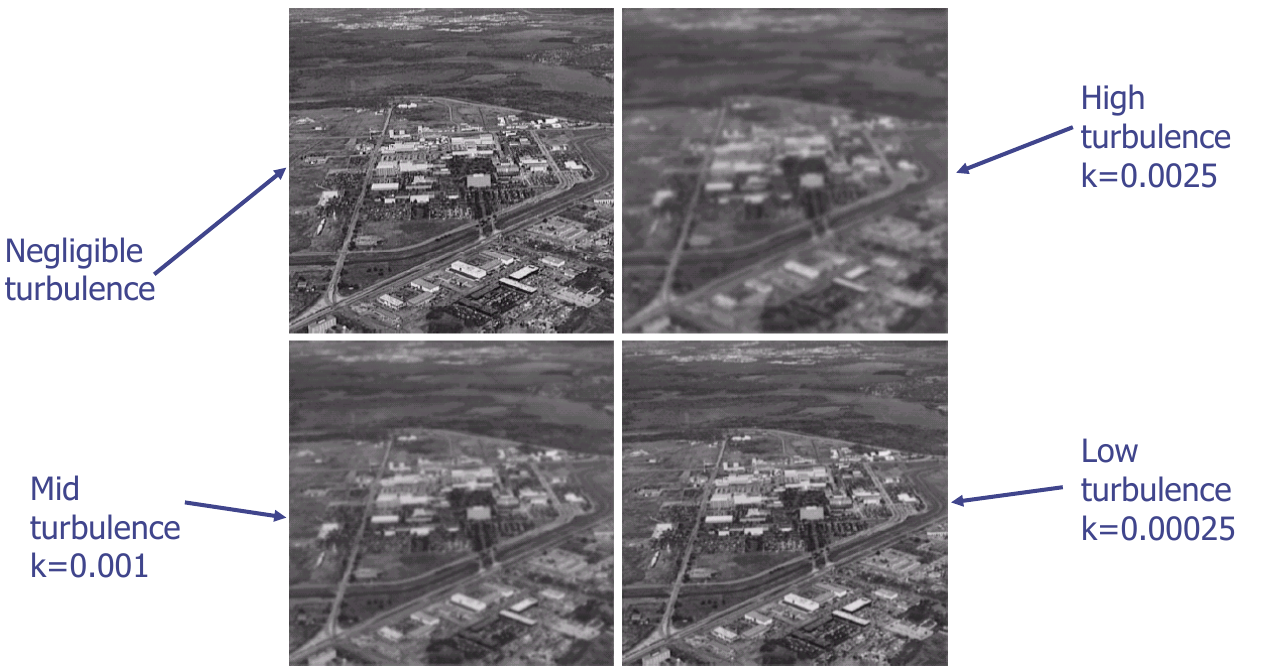
\includegraphics[scale=0.25]{images/L5_ex_Dm_turbelence.png}}
	\end{itemize}
}
\end{block}
\end{frame}
%-----------
\begin{frame}
\frametitle{Estimating the degradation function}
\begin{block}{Estimation by modeling}

\begin{itemize}
	\item Blurring by linear motion:  
	$$g(x,y) = \int^{T}_{0} f[x-x_{0}(t), y-y_{0}(t)] dt$$
	$$G(u,v) = F(u,v)\int^{T}_{0} e^{-j2\pi[ux_{0}(t)+vy_{0}(t)]} dt$$
	$$ \Rightarrow H(u,v) = \int^{T}_{0} e^{-j2\pi[ux_{0}(t)+vy_{0}(t)]} dt$$ 
	\item if $x_{0}(t) = at/T$ and $y_{0} = 0$ $\Rightarrow$
	$$H(u,v) = \int^{T}_{0} e^{-j2\pi uat/T} dt = \frac{T}{\pi ua} \sin(\pi ua) e^{-j\pi ua}  $$
	\end{itemize}
		
\end{block}
\end{frame}
%-----------
\begin{frame}
\frametitle{Estimating the degradation function}
\begin{block}{Estimation by modeling}
\begin{itemize}
\item if $x_{0}(t) = at/T$ and $y_{0} = bt/T$ $\Rightarrow$
    $$H(u,v) = \frac{T}{\pi (ua+vb)} \sin[\pi(ua+vb)] e^{-j\pi(ua+vb)}  $$
\item Result of motion blur wit $a= b= 0.1$ and $T = 1$
\item[]
\centering{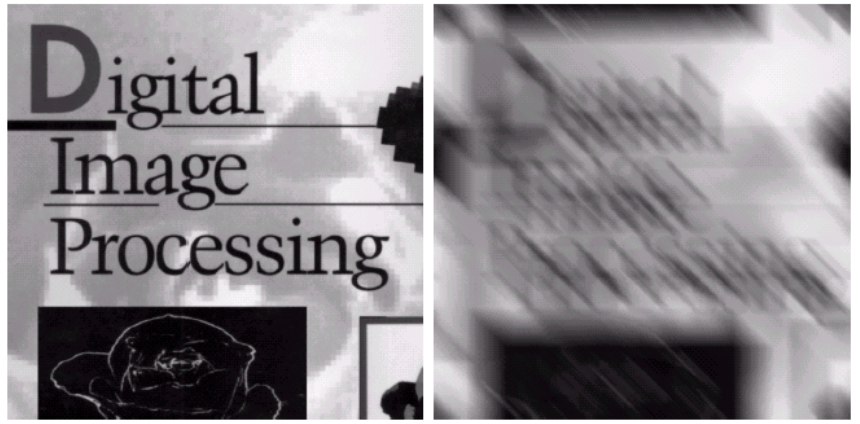
\includegraphics[scale=0.2]{images/L5-ex-motionblur.png}}    
\end{itemize}
\end{block}
\end{frame}
%-----------
\section{Inverse Filtering}
\begin{frame}
\frametitle{Inverse Filtering}
\begin{itemize}
\item The simplest form of restoration, direct inverse filtering  
$$\hat{F}(u,v) = \frac{G(u,v)}{H(u,v)} = F(u,v) + \frac{N(u,v)}{H(u,v)}$$
\end{itemize}

\begin{block}{Problems!!}
\scriptsize{
\begin{itemize}
\item Since $N(u,v)$ is un-known, even if we know the degradation function, the undegraded image cannot be recovered
\item  If $H(u,v)\simeq 0$, $N(u,v)/H(u,v)$  dominates the estimate of $\hat{F}(u,v)$
\end{itemize}
}
\end{block}
\begin{block}{Solutions-1}
\scriptsize{
\begin{itemize}
\item  Limiting the filter frequencies to value near origin, in order to get around the zero or small value problem 
\end{itemize}
}
\end{block}
\end{frame}
%-----------
\begin{frame}
\frametitle{Inverse Filtering}
\centering{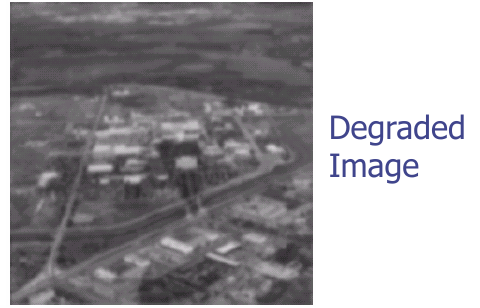
\includegraphics[scale=0.25]{images/L5_ex_IF_LF1.png}}\\
\centering{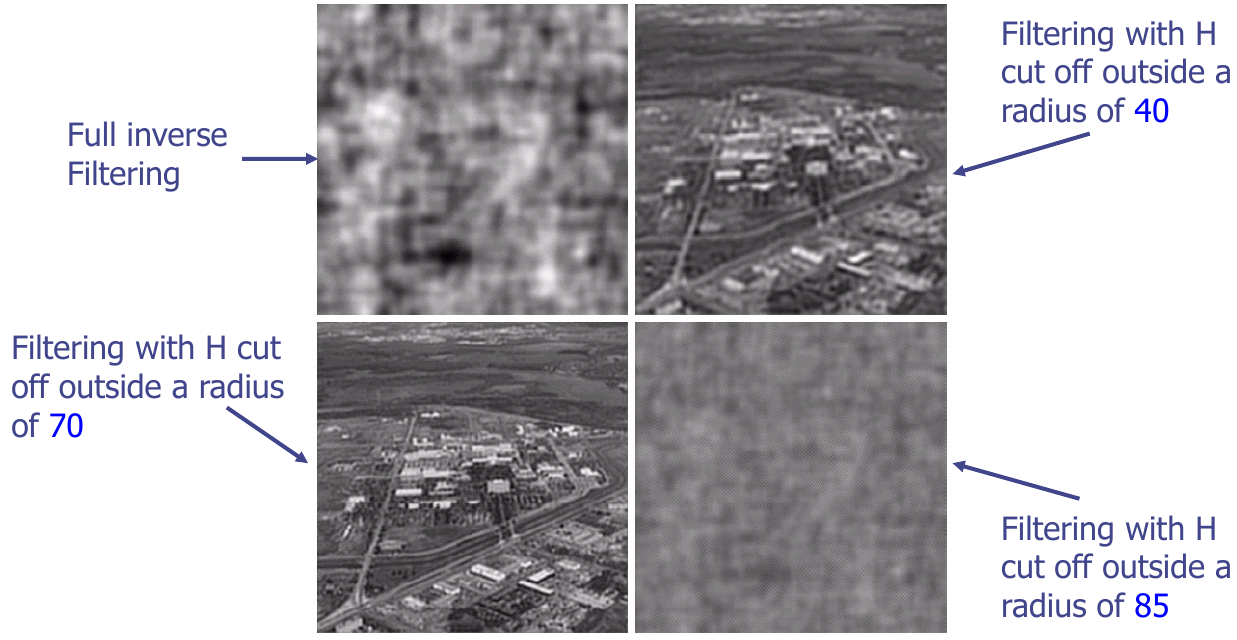
\includegraphics[scale=0.25]{images/L5_ex_IF_LF2.png}}
\end{frame}
%----------
\begin{frame}
\frametitle{Inverse Filtering}
\begin{block}{Solutions-2}
\begin{itemize}
\item If $H$ has zero elements, then at those frequencies the inverse filter does not exist, thus use the following inverting equation:
\[ \frac{H^{\ast}(u,v)}{H^{\ast}(u,v)H(u,v)+C} \approx 
	\begin{cases} 
   	H^{-1}(u,v) & \text{for } \vert H(u,v) \vert^{2} \gg C   \\
   	\frac{1}{c} H^{\ast}(u,v) & \text{for } \vert H(u,v) \vert^{2} \ll c
  	\end{cases}	
  	\]
\item Scaling the image at high frequencies by $\frac{1}{c}$ 
\item Simple example:\\

\centering{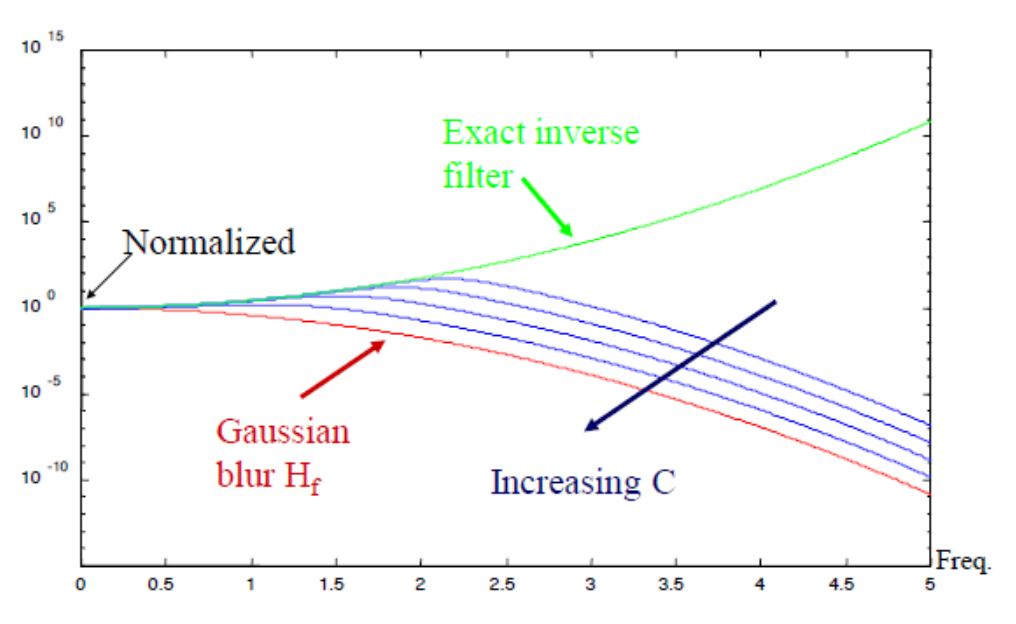
\includegraphics[scale=0.15]{images/L5_ex_IF_s2.png}}
\end{itemize}
\end{block}
\end{frame}
%-----------
\begin{frame}
\frametitle{Inverse Filtering}
\begin{block}{Solution-2}
\centering{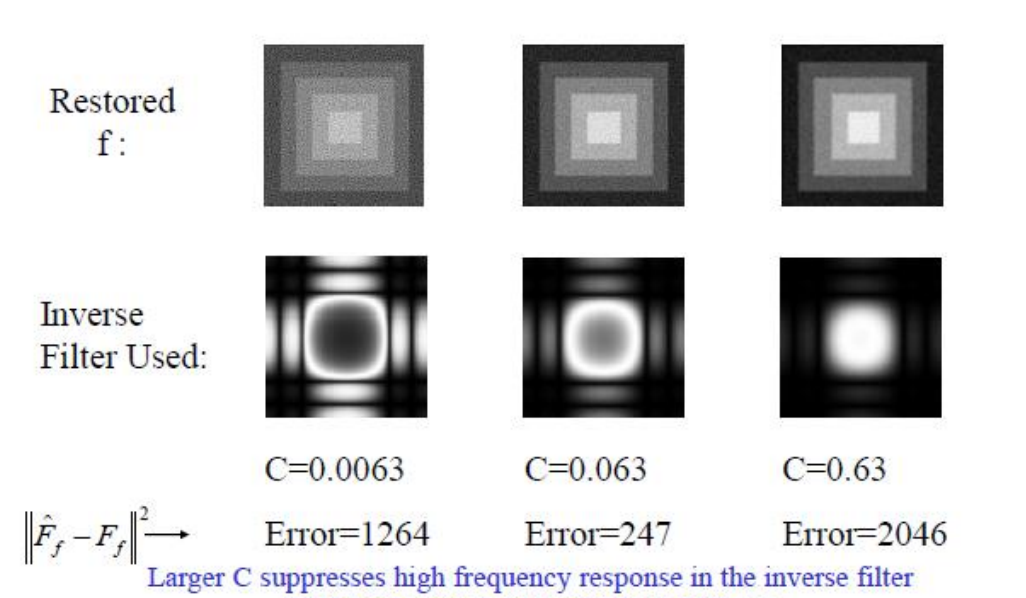
\includegraphics[scale=0.38]{images/L5_ex_IF_s2_2.png}}
\end{block}
\end{frame}
%-----------
\begin{frame}
\frametitle{Inverse Filtering}
\begin{block}{Solution-2}
{\color{blue} What is the best choice for $C$?}\\
\centering{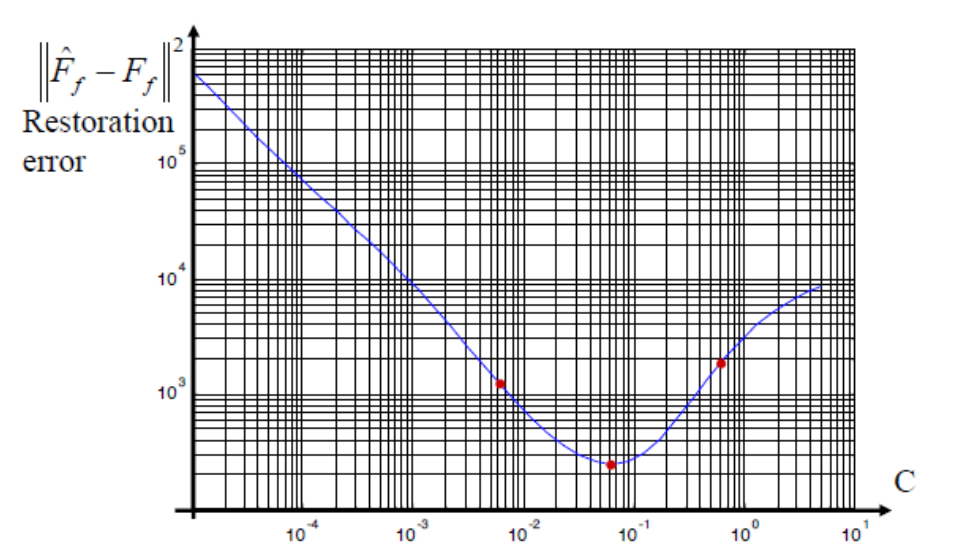
\includegraphics[scale=0.38]{images/L5_IF_s2_BC.png}}\\
{\color{blue}It is not a practical way !!}\\
\end{block}
\end{frame}
%-----------
\begin{frame}
\frametitle{Inverse Filtering}
\begin{block}{Solution-2}
\begin{itemize}
\item Drawbacks of this approach: 
\begin{itemize}
	\item Finding the best $C$ is not 
	\item $C$ is constant for all the frequencies, maybe it should be frequency dependent
	\item For high frequencies, where noise is dominant, the image is amplified by $1/C \gg 1$ $\Rightarrow$ amplifying the noise
\end{itemize}
\item Different strategies:
\begin{itemize}
	\item Same as before based on $H(u,v)$
	\begin{itemize}
		\item Where $H(u,v)$ is high apply the exact inverse, and where low apply $H_{f}/C$
	\end{itemize}	 
	\item Based on $SNR^{\ast}H(u,v)$
	\begin{itemize}
		\item $\vert H(u,v)\vert SNR \gg 1$ $\Rightarrow$ inverse
		\item $\vert H(u,v)\vert SNR \ll 1$ $\Rightarrow$ 0
	\end{itemize}	 
	\item Signal/Noise = $SNR^{2}$ = $\frac{\vert F(u, v) \vert^{2}}{\sigma^{2}}$	
\end{itemize}

\end{itemize}
\end{block}
\end{frame}


%-----------
\section{Wiener Filter}
\begin{frame}
\frametitle{Wiener Filter}
\begin{itemize}
\item Incorporates both the degradation function and statistical characteristics of noise into the restoration process
\item Objective is to find an estimate $\hat{f}$ of the uncorrupted image $f$, such that mean-square-error (MSR) between then is minimum
$$e^{2} = E{(f - \hat{f})^{2}} $$
\item Assumptions:
\begin{itemize}
	\item Noise and image are uncorrelated
	\item One or the other has zero mean
	\item The gray levels in the estimate are a linear function of the levels in the degradation image
\end{itemize}
\item The minimum of the error function in Frequency domain:
$$\hat{F}(u,v) = [\frac{1}{H(u,v)}\frac{\vert H(u,v) \vert^{2}}{\vert H(u,v) \vert^{2} + S_{\eta}(u,v)/S_{f}(u,v)}]G(u,v)$$
 
\end{itemize}
\end{frame}
%-----------
\begin{frame}
\frametitle{Wiener Filter \small{(minimum mean square error filter)}}
\begin{itemize}
\item[] $$\hat{F}(u,v) = [\frac{1}{H(u,v)}\frac{\vert H(u,v) \vert^{2}}{\vert H(u,v) \vert^{2} + S_{\eta}(u,v)/S_{f}(u,v)}]G(u,v)$$
\item $H(u,v)$, degradation function 
\item $H^{\ast}(u,v)$, complex conjugate of $H(u,v)$
\item $\vert H(u,v) \vert^{2} = H^{\ast}(u,v)H(u,v)$
\item $S_{\eta}(u,v) = \vert N(u,v) \vert^{2} $, power spectrum of the noise 
\item $S_{f}(u,v) = \vert F(u,v) \vert^{2} $, power spectrum of the undegraded image 
 
\end{itemize}
\end{frame}
%----------
\begin{frame}
\frametitle{Wiener Filter \small{(minimum mean square error filter)}}
\begin{itemize}
\scriptsize{
\item Signal-to-noise ratio (SNR)
$$SNR =\frac{\sum\limits^{M-1}_{u=0}\sum\limits^{N-1}_{v=0} \vert F(u,v)\vert^{2}}{\sum\limits^{M-1}_{u=0}\sum\limits^{N-1}_{v=0} \vert N(u,v)\vert^{2}} $$
\item Low noise $\rightarrow$ high SNR , high noise $\rightarrow$ low SNR
\item If we consider restored image $\hat{f}(x,y)$ to be \textbf{signal} and the difference between this image and the original image, \textbf{noise}: 
$$SNR = \frac{\sum\limits^{M-1}_{x=0}\sum\limits^{N-1}_{y=0} \hat{f}(x,y)^{2}}{\sum\limits^{M-1}_{x=0}\sum\limits^{N-1}_{y=0}[f(x,y)-\hat{f}(x,y))]^{2}} $$
\item Closer $f$ and $\hat{f}$, this ration is higher}
\end{itemize}
\end{frame}
%-----------
\begin{frame}
\frametitle{Wiener Filter \small{(minimum mean square error filter)}}
\begin{itemize}
\item Full inverse filtering, radially limited inverse filtering, and Wiener filtering, respectively
\item[]
\centering{
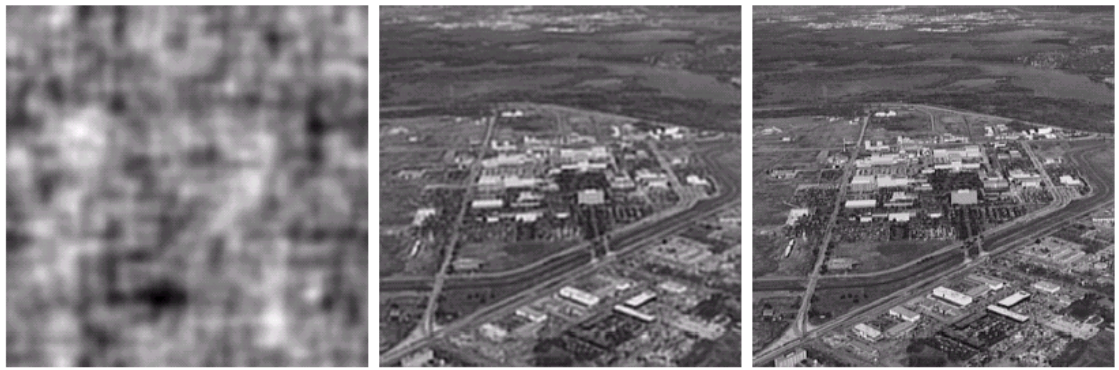
\includegraphics[scale=0.3]{images/L5_ex_Wiener.png}}
\end{itemize}
\end{frame}


%-----------
\end{document}

%\begin{itemize}
%\item Also use neighborhood but do not use coefficients 
%\begin{itemize}
%\item median filter for noise reduction
%\end{itemize} 
%\end{itemize}
